\PassOptionsToPackage{unicode=true}{hyperref} % options for packages loaded elsewhere
\PassOptionsToPackage{hyphens}{url}
%
\documentclass[]{article}
\usepackage{lmodern}
\usepackage{amssymb,amsmath}
\usepackage{ifxetex,ifluatex}
\usepackage{fixltx2e} % provides \textsubscript
\ifnum 0\ifxetex 1\fi\ifluatex 1\fi=0 % if pdftex
  \usepackage[T1]{fontenc}
  \usepackage[utf8]{inputenc}
  \usepackage{textcomp} % provides euro and other symbols
\else % if luatex or xelatex
  \usepackage{unicode-math}
  \defaultfontfeatures{Ligatures=TeX,Scale=MatchLowercase}
\fi
% use upquote if available, for straight quotes in verbatim environments
\IfFileExists{upquote.sty}{\usepackage{upquote}}{}
% use microtype if available
\IfFileExists{microtype.sty}{%
\usepackage[]{microtype}
\UseMicrotypeSet[protrusion]{basicmath} % disable protrusion for tt fonts
}{}
\IfFileExists{parskip.sty}{%
\usepackage{parskip}
}{% else
\setlength{\parindent}{0pt}
\setlength{\parskip}{6pt plus 2pt minus 1pt}
}
\usepackage{hyperref}
\hypersetup{
            pdftitle={On the Road and R Meets Python},
            pdfauthor={Ethan Pieniazek},
            pdfborder={0 0 0},
            breaklinks=true}
\urlstyle{same}  % don't use monospace font for urls
\usepackage[margin=1in]{geometry}
\usepackage{color}
\usepackage{fancyvrb}
\newcommand{\VerbBar}{|}
\newcommand{\VERB}{\Verb[commandchars=\\\{\}]}
\DefineVerbatimEnvironment{Highlighting}{Verbatim}{commandchars=\\\{\}}
% Add ',fontsize=\small' for more characters per line
\usepackage{framed}
\definecolor{shadecolor}{RGB}{248,248,248}
\newenvironment{Shaded}{\begin{snugshade}}{\end{snugshade}}
\newcommand{\AlertTok}[1]{\textcolor[rgb]{0.94,0.16,0.16}{#1}}
\newcommand{\AnnotationTok}[1]{\textcolor[rgb]{0.56,0.35,0.01}{\textbf{\textit{#1}}}}
\newcommand{\AttributeTok}[1]{\textcolor[rgb]{0.77,0.63,0.00}{#1}}
\newcommand{\BaseNTok}[1]{\textcolor[rgb]{0.00,0.00,0.81}{#1}}
\newcommand{\BuiltInTok}[1]{#1}
\newcommand{\CharTok}[1]{\textcolor[rgb]{0.31,0.60,0.02}{#1}}
\newcommand{\CommentTok}[1]{\textcolor[rgb]{0.56,0.35,0.01}{\textit{#1}}}
\newcommand{\CommentVarTok}[1]{\textcolor[rgb]{0.56,0.35,0.01}{\textbf{\textit{#1}}}}
\newcommand{\ConstantTok}[1]{\textcolor[rgb]{0.00,0.00,0.00}{#1}}
\newcommand{\ControlFlowTok}[1]{\textcolor[rgb]{0.13,0.29,0.53}{\textbf{#1}}}
\newcommand{\DataTypeTok}[1]{\textcolor[rgb]{0.13,0.29,0.53}{#1}}
\newcommand{\DecValTok}[1]{\textcolor[rgb]{0.00,0.00,0.81}{#1}}
\newcommand{\DocumentationTok}[1]{\textcolor[rgb]{0.56,0.35,0.01}{\textbf{\textit{#1}}}}
\newcommand{\ErrorTok}[1]{\textcolor[rgb]{0.64,0.00,0.00}{\textbf{#1}}}
\newcommand{\ExtensionTok}[1]{#1}
\newcommand{\FloatTok}[1]{\textcolor[rgb]{0.00,0.00,0.81}{#1}}
\newcommand{\FunctionTok}[1]{\textcolor[rgb]{0.00,0.00,0.00}{#1}}
\newcommand{\ImportTok}[1]{#1}
\newcommand{\InformationTok}[1]{\textcolor[rgb]{0.56,0.35,0.01}{\textbf{\textit{#1}}}}
\newcommand{\KeywordTok}[1]{\textcolor[rgb]{0.13,0.29,0.53}{\textbf{#1}}}
\newcommand{\NormalTok}[1]{#1}
\newcommand{\OperatorTok}[1]{\textcolor[rgb]{0.81,0.36,0.00}{\textbf{#1}}}
\newcommand{\OtherTok}[1]{\textcolor[rgb]{0.56,0.35,0.01}{#1}}
\newcommand{\PreprocessorTok}[1]{\textcolor[rgb]{0.56,0.35,0.01}{\textit{#1}}}
\newcommand{\RegionMarkerTok}[1]{#1}
\newcommand{\SpecialCharTok}[1]{\textcolor[rgb]{0.00,0.00,0.00}{#1}}
\newcommand{\SpecialStringTok}[1]{\textcolor[rgb]{0.31,0.60,0.02}{#1}}
\newcommand{\StringTok}[1]{\textcolor[rgb]{0.31,0.60,0.02}{#1}}
\newcommand{\VariableTok}[1]{\textcolor[rgb]{0.00,0.00,0.00}{#1}}
\newcommand{\VerbatimStringTok}[1]{\textcolor[rgb]{0.31,0.60,0.02}{#1}}
\newcommand{\WarningTok}[1]{\textcolor[rgb]{0.56,0.35,0.01}{\textbf{\textit{#1}}}}
\usepackage{graphicx,grffile}
\makeatletter
\def\maxwidth{\ifdim\Gin@nat@width>\linewidth\linewidth\else\Gin@nat@width\fi}
\def\maxheight{\ifdim\Gin@nat@height>\textheight\textheight\else\Gin@nat@height\fi}
\makeatother
% Scale images if necessary, so that they will not overflow the page
% margins by default, and it is still possible to overwrite the defaults
% using explicit options in \includegraphics[width, height, ...]{}
\setkeys{Gin}{width=\maxwidth,height=\maxheight,keepaspectratio}
\setlength{\emergencystretch}{3em}  % prevent overfull lines
\providecommand{\tightlist}{%
  \setlength{\itemsep}{0pt}\setlength{\parskip}{0pt}}
\setcounter{secnumdepth}{0}
% Redefines (sub)paragraphs to behave more like sections
\ifx\paragraph\undefined\else
\let\oldparagraph\paragraph
\renewcommand{\paragraph}[1]{\oldparagraph{#1}\mbox{}}
\fi
\ifx\subparagraph\undefined\else
\let\oldsubparagraph\subparagraph
\renewcommand{\subparagraph}[1]{\oldsubparagraph{#1}\mbox{}}
\fi

% set default figure placement to htbp
\makeatletter
\def\fps@figure{htbp}
\makeatother


\title{On the Road and R Meets Python}
\author{Ethan Pieniazek}
\date{2020-05-14}

\begin{document}
\maketitle

\hypertarget{the-last-two-months}{%
\subsection{\texorpdfstring{\textbf{The Last Two
Months}}{The Last Two Months}}\label{the-last-two-months}}

\emph{The past couple months have been very interesting to say the
least. After spring break got extended an extra week, my buddy Robbie
and I decided to extend our stay in Red Rock near Las Vegas another week
to climb the sandstone. Halfway through the trip I received news that
campus had been closed and all classes were to be moved remotely via
Zoom. The official campsite right by Red Rock also shut down March 22nd
due to the virus, so we decided to hold it out another week in an area a
bit further away from Red Rock where we could dispersed camp and see if
school was feasible on the road, using my car as my office/charging port
and my phone as a hotspot. It ended up working out just fine even though
there were many problems to figure out along the way. Some of these
problems included where we were going to shower now that businesses were
closed, where we would fill up water, where to efficiently buy
groceries, and where to find better places to camp that were closer to
Red Rock (which we eventually found due to word of mouth from other
climbers). Staying in Las Vegas ended up being well worth it as all the
classic lines people are often found waiting in line for or even worse
`congalining' were all empty since the Red Rock Scenic Loop that makes
the conservation area easily accessible was closed. Long approaches of
up to 2 hours became the norm on days we climbed, but the reward was
getting to an area that is often just too busy and having it completely
vacant. It truly felt like a once in a lifetime experience and we are
glad we stayed in Vegas until it got too hot to continue. We are
currently at Mount Lemmon just outside of Tucson, Arizona. Even though
Tucson has high temperatures this time of year, Mount Lemmon
consistently stays around 30 degrees cooler. Cragging along the Catalina
Highway has been great as the approaches are much shorter and we do not
have to take our tent down every morning. Packing in all our water for
the week in a sedan along with packing out all of our trash back to
Tucson gets tricky sometimes, but we make it work with a couple trips to
town every week. It is nice to climb on the different rock here being
granite as limestone is practically all there is in Austin besides the
pink granite domes at Enchanted Rock. Even though commencement got
delayed it was cool this situation came from it as I would have never
anticipated dirtbagging my last semester of college.}
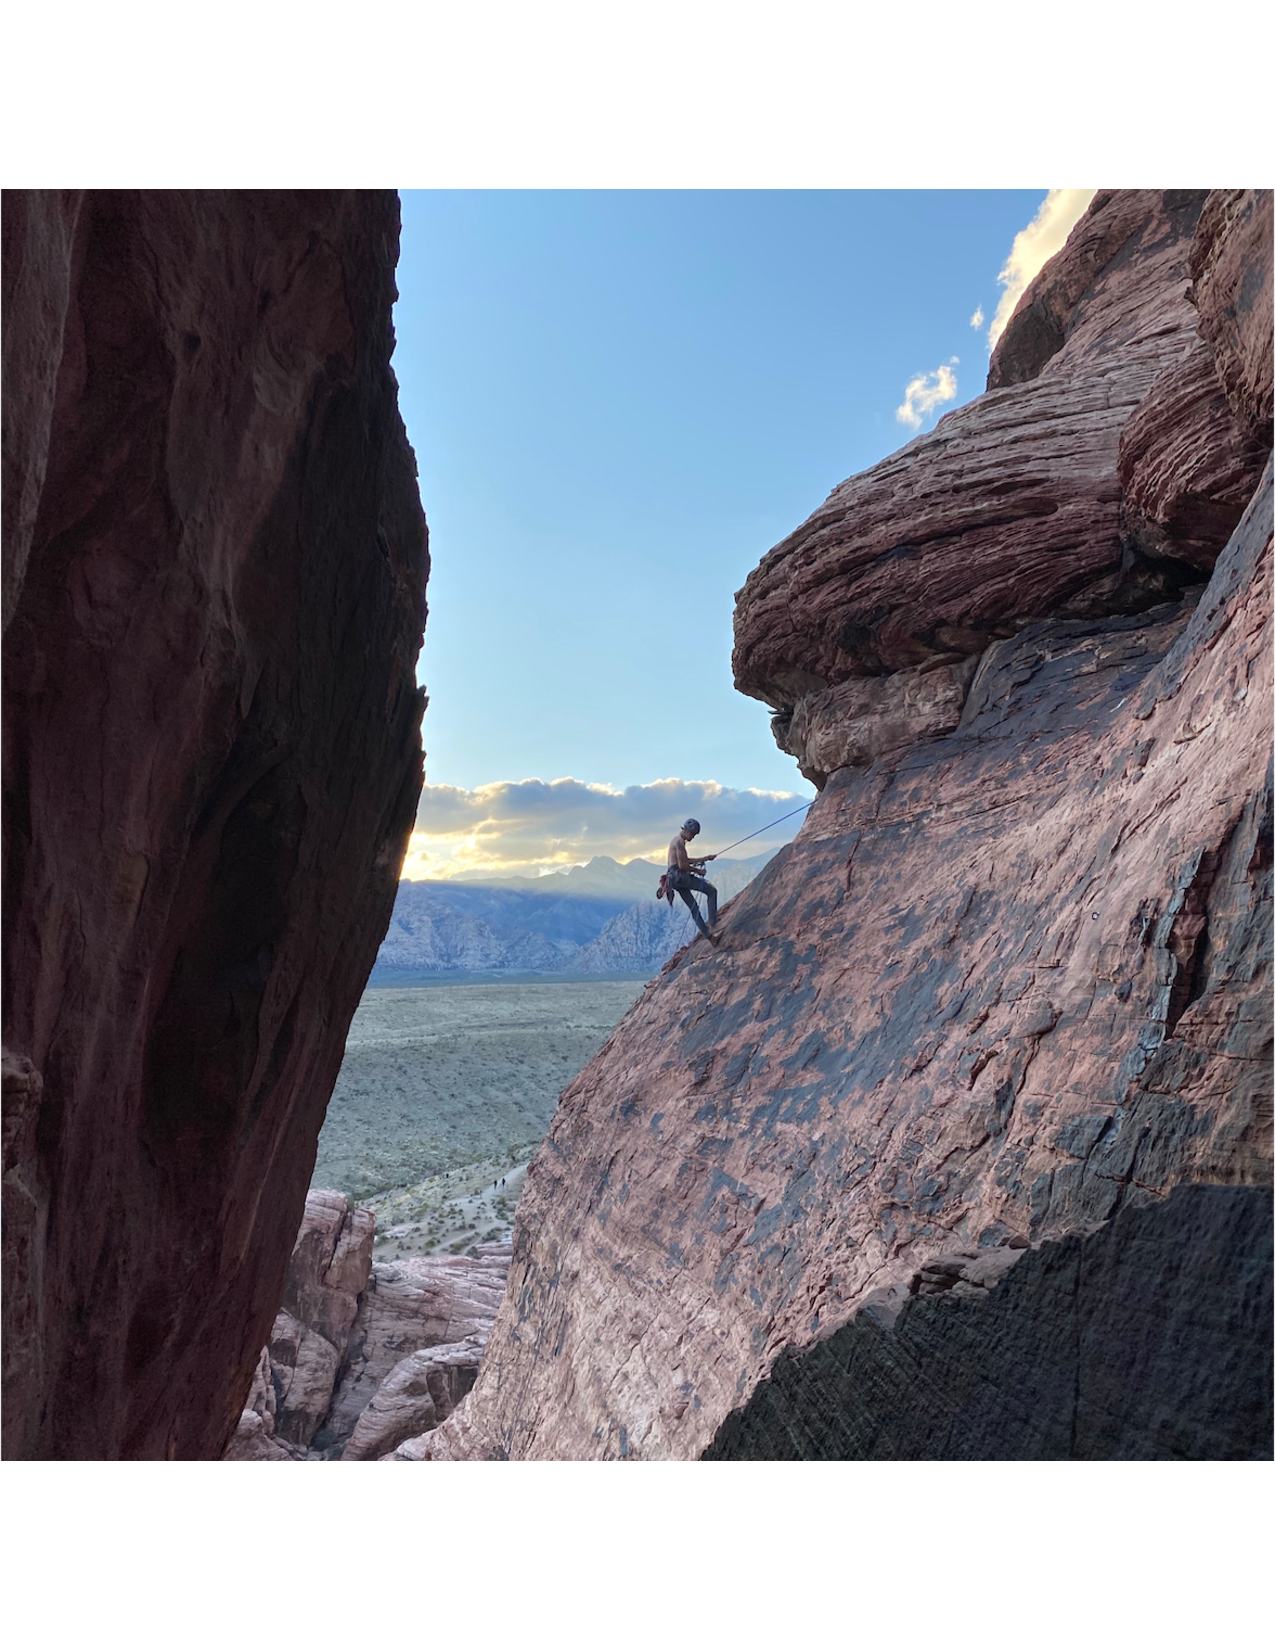
\includegraphics{/blog/2020-05-14-dirtbagging-and-r-meets-python_files/rrock.png}

\hypertarget{r-meets-python}{%
\subsection{\texorpdfstring{\textbf{R meets
Python}}{R meets Python}}\label{r-meets-python}}

\emph{During my last semester for my computational biology class I spend
lots of time learning the fundamentals of R, the various packages that
make calculating statistics/creating plots much more efficient, and how
to showcase these skills with data scavenged from the real world. It
turned out to be one of the coolest classes I have taken at UT as it
taught me how to exhaust my resources in order to find the answer to the
question at stake. I quickly found what I liked so much about coding in
R being that one does not have to learn everything at once or even in
any particular order. It is rather all about finding what you need for a
particular project, implementing it, and then being able to access the
information next time to help with other projects. As I kept messing
around with R I kept learning more and more about how to troubleshoot
future problems quicker and more efficiently. It was cool to find
something that could keep me busy without getting distracted for hours
on end until I found the solution.}

\emph{Just as R started to become something I felt much more ``fluent''
in, Python came around. At first Python seemed so much different than R.
Indexing was new and weird as now the first character in an array was in
the zeroth position, the syntax as much different, and the interface
(even on Jupyterhub) was not as inviting as R Studio. It was cool to
learn R before Python came into the picture though because it made
understanding the new language easier to comprehend and adjust to. One
of the coolest topics we learned was how to use regular expressions
(Regex) to find and print sequences and patterns from a string. Regex is
particularly important for data science since it allows one to extract
for example URLs, numbers, IP addresses, names, etc. In genetics it has
become increasingly important with DNA sequencing as a major tool for
sorting through a given sequence. In the example below from one of the
assignments this semester, I will show how Regex can be implemented for
biological purposes.}

\emph{In the string below we want to find the sites that match the
enzyme binding sites for GCRWTG and ANTAAT where N is any base, R is A
or G and W is A or T. The regex `findall' operation was used to search
the sequence for the enzyme binding sites of interest. For the first
site `GCRWTG' the first two bases had to be GC so that is why these
bases are first in the expression. The next base could either be an A or
G so `{[}{]}' were used to search the string for GC followed by an A or
G. The same goes for the next base as it had to be either an A or T.
Since the last two bases were TG this was specified at the end of the
expression for this first binding site. The `\textbar{}' was then used
to search for another enzyme binding site `ANTAAT'. This was even more
straight forward since the only base that could differ was the second
where it could be any base. The `.' was used to include any other
character after A since N could be any nucleotide. The rest of the
expression made it so that only the first two bases followed by TAAT
would be included in the output. After running the code, the result was
four fragments matching the criteria for the regular expression. }

\begin{Shaded}
\begin{Highlighting}[]
\ImportTok{import}\NormalTok{ numpy }\ImportTok{as}\NormalTok{ mp}
\ImportTok{import}\NormalTok{ re }\ImportTok{as}\NormalTok{ re}
\NormalTok{string5 }\OperatorTok{=} \StringTok{"ATGGCAATAACCCCCCGTTTCTACTTCTAGAGGAGAAAAGTATTGACATGAGCGCTCCCGGCACAAGGGCCAAAGAAGTCTCCAATTTCTTATTTCCGAATGACATGCGTCTCCTTGCGGGTAAATCACCGACCGCAATTCATAGAAGCCTGGGGGAACAGATAGGTCTAATTAGCTTAAGAGAGTAAATCCTGGGATCATTCAGTAGTAACCATAAACTTACGCTGGGGCTTCTTCGGCGGATTTTTACAGTTACCAACCAGGAGATTTGAAGTAAATCAGTTGAGGATTTAGCCGCGCTATCCGGTAATCTCCAAATTAAAACATACCGTTCCATGAAGGCTAGAATTACTTACCGGCCTTTTCCATGCCTGCGCTATACCCCCCCACTCTCCCGCTTATCCGTCCGAGCGGAGGCAGTGCGATCCTCCGTTAAGATATTCTTACGTGTGACGTAGCTATGTATTTTGCAGAGCTGGCGAACGCGTTGAACACTTCACAGATGGTAGGGATTCGGGTAAAGGGCGTATAATTGGGGACTAACATAGGCGTAGACTACGATGGCGCCAACTCAATCGCAGCTCGAGCGCCCTGAATAACGTACTCATCTCAACTCATTCTCGGCAATCTACCGAGCGACTCGATTATCAACGGCTGTCTAGCAGTTCTAATCTTTTGCCAGCATCGTAATAGCCTCCAAGAGATTGATGATAGCTATCGGCACAGAACTGAGACGGCGCCGATGGATAGCGGACTTTCGGTCAACCACAATTCCCCACGGGACAGGTCCTGCGGTGCGCATCACTCTGAATGTACAAGCAACCCAAGTGGGCCGAGCCTGGACTCAGCTGGTTCCTGCGTGAGCTCGAGACTCGGGATGACAGCTCTTTAAACATAGAGCGGGGGCGTCGAACGGTCGAGAAAGTCATAGTACCTCGGGTACCAACTTACTCAGGTTATTGCTTGAAGCTGTACTATTTTAGGGGGGGAGCGCTGAAGGTCTCTTCTTCTCATGACTGAACTCGCGAGGGTCGTGAAGTCGGTTCCTTCAATGGTTAAAAAACAAAGGCTTACTGTGCGCAGAGGAACGCCCATCTAGCGGCTGGCGTCTTGAATGCTCGGTCCCCTTTGTCATTCCGGATTAATCCATTTCCCTCATTCACGAGCTTGCGAAGTCTACATTGGTATATGAATGCGACCTAGAAGAGGGCGCTTAAAATTGGCAGTGGTTGATGCTCTAAACTCCATTTGGTTTACTCGTGCATCACCGCGATAGGCTGACAAAGGTTTAACATTGAATAGCAAGGCACTTCCGGTCTCAATGAACGGCCGGGAAAGGTACGCGCGCGGTATGGGAGGATCAAGGGGCCAATAGAGAGGCTCCTCTCTCACTCGCTAGGAGGCAAATGTAAAACAATGGTTACTGCATCGATACATAAAACATGTCCATCGGTTGCCCAAAGTGTTAAGTGTCTATCACCCCTAGGGCCGTTTCCCGCATATAAACGCCAGGTTGTATCCGCATTTGATGCTACCGTGGATGAGTCTGCGTCGAGCGCGCCGCACGAATGTTGCAATGTATTGCATGAGTAGGGTTGACTAAGAGCCGTTAGATGCGTCGCTGTACTAATAGTTGTCGACAGACCGTCGAGATTAGAAAATGGTACCAGCATTTTCGGAGGTTCTCTAACTAGTATGGATTGCGGTGTCTTCACTGTGCTGCGGCTACCCATCGCCTGAAATCCAGCTGGTGTCAAGCCATCCCCTCTCCGGGACGCCGCATGTAGTGAAACATATACGTTGCACGGGTTCACCGCGGTCCGTTCTGAGTCGACCAAGGACACAATCGAGCTCCGATCCGTACCCTCGACAAACTTGTACCCGACCCCCGGAGCTTGCCAGCTCCTCGGGTATCATGGAGCCTGTGGTATCATCGCGTCCGATATCAAACTTCGTCATGATAAAGTCCCCCCCTCGGGAGTACCAGAGAAGATGACTACTGAGTTGTGCGAT"}
\NormalTok{re.findall(}\VerbatimStringTok{r'GC[AG][AT]TG|A.TAAT'}\NormalTok{,string5)}
\end{Highlighting}
\end{Shaded}

\begin{verbatim}
## ['GCGTTG', 'ATTAAT', 'GCAATG', 'ACTAAT']
\end{verbatim}

\end{document}
